% NeurIPS 2026 MLxOR workshop short paper (single-blind, non-anonymous).
\documentclass{article}

\usepackage[sglblindworkshop]{neurips_2026}
\workshoptitle{MLxOR}
\usepackage{amsmath,amssymb,booktabs,graphicx,microtype,url}
\graphicspath{{../results/figures/}}

\title{Does Bellman-Residual Feedback Help Adaptive State Aggregation?\\
A Controlled Negative Result}

\author{%
  Sunny Zhang\\
  University of Toronto\\
  \texttt{ssunny.zhang@mail.utoronto.ca}
}

\newcommand{\err}{\operatorname{err}_{\infty}}
\newcommand{\R}{\textsc{Residual}}
\newcommand{\G}{\textsc{Geometric}}
\newcommand{\F}{\textsc{Fixed}}
\newcommand{\VI}{\textsc{VI}}

\begin{document}

\maketitle

\begin{abstract}
Adaptive state aggregation replaces full-state Bellman updates with updates on
groups of states having similar values.  A natural refinement rule shrinks the
group width in response to the Bellman residual, but any gain may come from
annealing itself rather than from feedback.  We isolate these effects on a
9,261-state inventory-control MDP by comparing
$\varepsilon_t=\max\{0.05,0.084\,\operatorname{span}(TV_t-V_t)\}$ with a
geometric timetable matched in initial width, floor, and decay rate.  Across
three global/aggregate update mixes and 20 paired sampling seeds, every 95\%
bootstrap interval for the final residual-minus-geometric value error lies
inside a preregistered $\pm0.02$ practical-equivalence region.  Residual
feedback is never practically better; in the global-heavy mix it is slightly
worse ($+0.00632$), although policy-loss rankings disagree with value-error
rankings.  Full-state value iteration also reaches the ground-truth stopping
tolerance in fewer charged backups.  This case study suggests that the useful
ingredient is a refinement timetable, not residual feedback, and illustrates
why adaptive dynamic programming should be evaluated against open-loop and
decision-quality controls.
\end{abstract}

\section{Introduction}

State aggregation combats the state-space cost of dynamic programming by
solving a smaller surrogate MDP \citep{whitt1978,bertsekas1989,li2006}.  In the
adaptive scheme of \citet{chen2021}, states with nearby current values share a
group, and ordinary Bellman sweeps alternate with stochastic group sweeps.  A
fixed bin width $\varepsilon$ creates a familiar cost--accuracy tradeoff: coarse
groups are cheap but impose approximation error, while fine groups preserve
accuracy but perform more backups.

This invites a feedback controller.  When the Bellman residual is large, a
coarse representation may suffice; as the residual contracts, the algorithm
can refine.  The key identification problem is that feedback also creates an
annealing schedule.  Comparing it only with a fixed width cannot tell whether
the residual signal helps or whether almost any schedule with the same decay
would work.

We test the signal itself.  A residual-driven rule is compared with an
open-loop geometric control matched in starting width, floor, and approximate
time to the floor.  The original experiment was preregistered at one update mix
and a 20\,ms endpoint.  We preserve that result, including the endpoint's
failure, and add a work-indexed robustness check at three update mixes.  The
result is negative but operationally useful: residual feedback provides no
practical improvement over the matched timetable on this instance.  Exact
rankings instead depend on update allocation and on whether performance is
measured by value error or decision loss.

\paragraph{Relation to prior work.}
Classical aggregation analyses bound the loss from replacing a dynamic program
with a smaller one \citep{whitt1978}; adaptive methods additionally change the
aggregation directions or groups as computation proceeds \citep{bertsekas1989}.
State-abstraction theory distinguishes several notions of when ground states
may safely share an abstract state \citep{li2006}.  We study the especially
simple value-based construction of \citet{chen2021}, whose guarantee scales as
$2\varepsilon/(1-\gamma)$ when states in a group differ by at most
$\varepsilon$.  Our question is complementary to those approximation results.
We do not propose a new abstraction or convergence theorem; we ask whether a
particular feedback signal improves the finite-compute trajectory after its
induced annealing path is controlled for.

\section{Method}

For a finite discounted cost MDP, define
\begin{equation}
 (TV)(s)=\min_a\left[c(s,a)+\gamma\sum_{s'}P(s'\mid s,a)V(s')\right].
 \label{eq:bellman}
\end{equation}
The solver bins $V(s)$ into occupied intervals of width $\varepsilon$.  A
global iteration evaluates \eqref{eq:bellman} for every state.  An aggregate
iteration samples one state per group, performs one lifted Bellman backup for
that representative, and updates the group value with step size
$\alpha_t=1/\sqrt{t}$.  A schedule $(\ell_g,\ell_a)$ repeats $\ell_g$ global
and $\ell_a$ aggregate iterations.  Rebinning occurs on entry to each aggregate
phase, and lifting occurs on return to the global phase.

After each global sweep we record
$r_t=\operatorname{span}(TV_t-V_t)=\max_s(TV_t-V_t)(s)-
\min_s(TV_t-V_t)(s)$.  The tested feedback rule is
\begin{equation}
 \varepsilon_t^{\R}=\max\{\varepsilon_{\min},c r_t\},
 \qquad c=0.084,\quad \varepsilon_{\min}=0.05.
 \label{eq:residual}
\end{equation}
Its first finite width is $0.4985$ and it reaches the floor after roughly
14 aggregate entries.  The main control never reads $r_t$:
\begin{equation}
 \varepsilon_j^{\G}=\max\!\left\{\varepsilon_{\min},
 0.4985\left(\frac{\varepsilon_{\min}}{0.4985}\right)^{j/13}\right\}.
 \label{eq:geometric}
\end{equation}
Thus \R{} and fast \G{} differ primarily in closed-loop versus open-loop
refinement.  A fixed $\varepsilon=0.05$ arm tests whether refinement is useful
at all.  Slower geometric and coarser fixed controls are retained in the
artifact but are not needed for the central contrast.

\paragraph{Inventory MDP.}
A state is the inventory vector $q\in\{-10,\ldots,10\}^3$, giving
$|\mathcal S|=21^3=9{,}261$.  Five joint quote-aggressiveness actions have fill
probabilities $(.1,.2,.4,.6,.8)$ and spreads $(1,.8,.5,.3,.15)$.  A transition
is no fill or a one-unit fill on either side of one asset.  The one-period cost
combines spread revenue with correlated inventory risk,
$c(q,a)=0.02q^\top\Sigma q-\delta_a f_a L(q)$, where $\Sigma$ has unit diagonal
and correlation $0.5$, and $L(q)$ removes infeasible boundary fills.  We use
$\gamma=.95$ and rescale costs so $\lVert V^*\rVert_\infty=100$.  This is a
small market-making-style control model \citep{avellaneda2008}, not a calibrated
market simulator.

\paragraph{Protocol and metrics.}
Each arm runs 10,000 iterations at $(5,2)$, $(2,5)$, and $(1,20)$.  The MDP is
deterministic; seeds $0$--$19$ vary the within-group sampling stream and are
paired across arms.  The primary reported metric is
$\err=\lVert V-V^*\rVert_\infty$.  We also evaluate the greedy policy
$\pi_V$ by $\lVert V^{\pi_V}-V^*\rVert_\infty$.

Work-indexed curves use billed Bellman backups
$B=n_g|\mathcal S|+\sum_t K_t$, where $K_t$ is the number of occupied groups.
This accounting is favorable to aggregation: rebinning and lifting add
$(n_r+n_l)|\mathcal S|$ state operations, and the residual scan is not charged.
For final paired differences we report the median and a seeded 10,000-resample
percentile-bootstrap interval.  The preregistered practical-equivalence region
is $[-0.02,0.02]$ on the 100-normalized value scale.

\section{Results}

\begin{figure}[t]
  \centering
  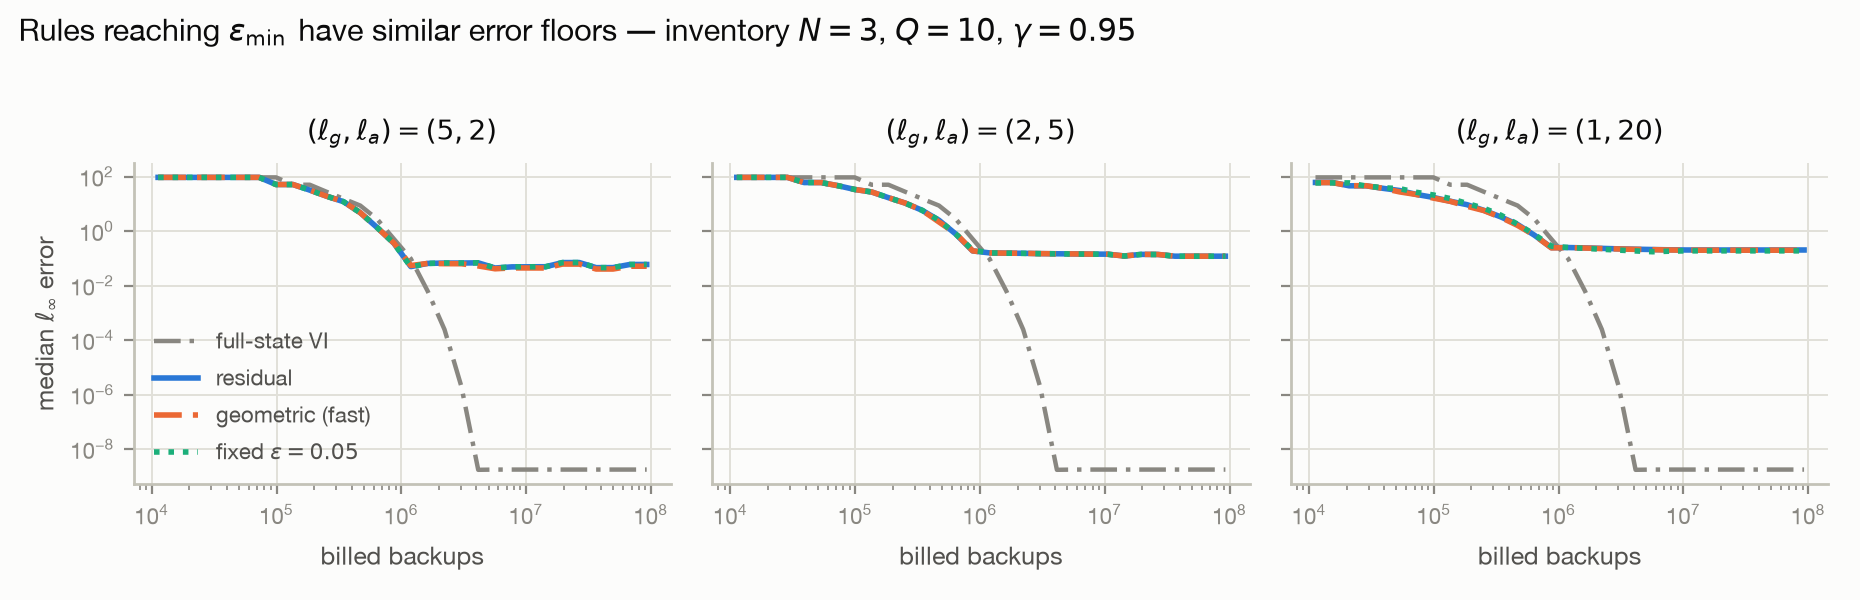
\includegraphics[width=\linewidth]{schedule_inventory_n3_light.png}
  \caption{Median value error against billed Bellman backups; terminal estimates
  are retained after an arm's 10,000-iteration horizon.  Curves for residual,
  fast geometric, and fixed-$0.05$ nearly coincide within each update mix.  The
  full-state \VI{} trajectory is deterministic and is repeated for reference;
  its convergence check stops after 454 sweeps (4.20M backups), although the
  plotted diagnostic continues to the common 10,000-sweep horizon.}
  \label{fig:curves}
\end{figure}

Figure~\ref{fig:curves} shows the central negative result.  Once the residual
and geometric rules reach $\varepsilon_{\min}$, their work--error trajectories
are visually inseparable at the plot scale.  Table~\ref{tab:final} makes the
small differences visible.  At all three mixes, the full paired interval for
residual minus fast geometric lies inside the $\pm0.02$ equivalence region.
At $(5,2)$ the interval excludes zero and every seed favors geometric in value
error, but the median difference is only $0.00632$.  At the preregistered
$(2,5)$ mix the median difference is $-2.9\times10^{-6}$, with an interval
straddling zero.  Residual feedback is therefore never practically better and
is sometimes detectably, though not practically, worse.

\begin{table}[t]
  \centering
  \small
  \setlength{\tabcolsep}{4.2pt}
  \caption{Final iterate over 20 paired seeds.  Columns R/G/F are residual,
  fast geometric, and fixed $\varepsilon=.05$.  The interval is for the median
  paired error difference R$-$G.  Policy loss is reported in the same order.}
  \label{tab:final}
  \begin{tabular}{@{}lrrrrl@{}}
    \toprule
    Mix & $\err(\mathrm R)$ & $\err(\mathrm G)$ & $\err(\mathrm F)$ & R$-$G (95\% CI)
      & Policy loss R/G/F \\
    \midrule
    $(5,2)$  & .05001 & .04368 & .05001 & .00632 [.00632,.00633]
      & .00210/.00278/.00210 \\
    $(2,5)$  & .13882 & .13882 & .13791 & $-$.000003 [$-$.000412,.000000]
      & .01518/.01609/.01280 \\
    $(1,20)$ & .20343 & .20053 & .19093 & $-$.00018 [$-$.00208,.00609]
      & .05178/.05178/.01649 \\
    \bottomrule
  \end{tabular}
\end{table}

The fixed control exposes two qualifications.  First, at $(1,20)$ residual is
worse than fixed-$0.05$ by $0.01250$ in value error (95\% CI
$[0.00745,0.01561]$) and by $0.03529$ in policy loss.  Second, value accuracy
does not order decision quality: at $(5,2)$ fast geometric has the lowest value
error but higher policy loss than residual, while at $(2,5)$ the slow geometric
arm (artifact only) has the lowest value error and 2.5 times fixed-$0.05$'s
policy loss.  Feedback cannot be justified by either metric here.

The mixes also consume different work.  Median residual billed backups are
67.68M, 30.21M, and 9.18M for $(5,2)$, $(2,5)$, and $(1,20)$; maintenance adds
39\%, 88\%, and 96\% respectively.  Hence the lower final error of the
global-heavy mix is not a causal ``schedule wins'' result: it purchases more
global work.  Full-state \VI{} is the sharper baseline.  The same implementation
meets its $10^{-10}$ update tolerance in 454 sweeps, or 4.20M billed backups,
and the 10,000-sweep diagnostic has $1.76\times10^{-9}$ error relative to the
cached solution.  On this instance, aggregation itself is not competitive;
the experiment identifies behavior inside an approximation scheme, not a new
best solver.

\paragraph{The preregistered endpoint failed.}
The original primary endpoint was $(2,5)$ at 20\,ms.  It gave a residual-minus-
geometric median of $-0.0417$ with 95\% CI $[-0.0459,0.0011]$, which is
indeterminate under the equivalence rule.  Worse, repeated executions changed
the interval because 20\,ms lies on a steep transient and selects a different
iterate as machine load changes.  We report rather than replace that outcome.
The final-iterate and backup-indexed analyses are explicitly robustness
analyses, motivated by this protocol failure, not retroactively preregistered
endpoints.

\section{What the negative result isolates}

\paragraph{Endpoint matching is load-bearing.}
A second geometric arm makes the control failure concrete.  The original slow
schedule used 1,429 aggregate cycles, exactly the number induced by 10,000
iterations at cycle length seven.  Transplanting it unchanged to $(1,20)$
provides only 477 aggregate entries: it ends at $\varepsilon=.232$ and error
$1.59$.  Recalibrating only its cycle count to 477 makes it end at
$\varepsilon=.05024$ and error $.209$, back in the neighborhood of residual
and fast geometric.  The apparent failure was caused by an unfinished
timetable, not by lack of feedback.  More generally, an open-loop control must
be matched in the clock on which adaptation occurs---here, aggregate entries,
not total iterations.

\paragraph{Equivalence is not equality.}
At $(5,2)$ the paired interval $[.006319,.006327]$ is exceptionally narrow and
excludes zero.  Calling the arms ``indistinguishable'' would therefore be
false.  The predeclared question was instead whether the entire interval lies
inside a practically negligible $\pm.02$ region; it does.  This distinction is
important for negative results with low simulation variance: abundant precision
can detect a difference too small to justify the adaptive mechanism.  Conversely,
the $(1,20)$ interval crosses zero but is wider.  Both satisfy the same practical
criterion for different statistical reasons.

\paragraph{Artifact and audit trail.}
The repository records the frozen residual constants and timing endpoint before
the residual arm was run, as well as the later schedule sweep, full configuration,
software environment, per-seed endpoints, paired differences, and work-indexed
curves.  Compiled and pure-Python tests check Bellman backups, partitions,
schedule semantics, seeded trajectories, and the $\ell_g=1,\ell_a=0$ reduction
to ordinary \VI{}.  The reported sweep used CPython 3.14.6, NumPy 2.4.6, and
Numba 0.67.0.  Code and data will be available at
\url{https://github.com/sunnysanitize/Residual-Epsilon-Aggregation}.

\section{Limitations and conclusion}

This study has one deterministic inventory instance, one residual statistic,
one floor, and stochasticity only from representative sampling.  The three
update mixes and backup endpoints were added after the preregistered timing
experiment.  Billed backups omit residual computation and representation
maintenance; charging them only strengthens \VI{} but may change comparisons
among aggregation schemes.  Policy loss is quantized by the finite action set,
and no claim is made about other MDPs, learned models, or settings where
aggregation is genuinely faster than \VI{}.  In particular, feedback could
matter when residuals are heterogeneous across regions, the useful floor is
unknown, or the horizon ends before every schedule reaches it.

Within this scope, however, the result is stable: across three update mixes,
Bellman-residual feedback never provides a practically meaningful improvement
over a matched open-loop timetable.  The broader methodological lesson is that
adaptive algorithms require controls that reproduce the path induced by their
feedback.  Otherwise, ordinary scheduling can be mistaken for intelligence.

\clearpage
\bibliographystyle{plainnat}
\begin{thebibliography}{9}

\bibitem[Avellaneda and Stoikov(2008)]{avellaneda2008}
Marco Avellaneda and Sasha Stoikov.
\newblock High-frequency trading in a limit order book.
\newblock \emph{Quantitative Finance}, 8(3):217--224, 2008.

\bibitem[Bertsekas and Castanon(1989)]{bertsekas1989}
Dimitri P. Bertsekas and David A. Castanon.
\newblock Adaptive aggregation methods for infinite horizon dynamic
  programming.
\newblock \emph{IEEE Transactions on Automatic Control}, 34(6):589--598, 1989.

\bibitem[Chen et~al.(2021)Chen, Gaebler, Peng, Sun, and Ye]{chen2021}
Guanting Chen, Johann Demetrio Gaebler, Matt Peng, Chunlin Sun, and Yinyu Ye.
\newblock An adaptive state aggregation algorithm for Markov decision
  processes.
\newblock \emph{arXiv preprint arXiv:2107.11053}, 2021.

\bibitem[Li et~al.(2006)Li, Walsh, and Littman]{li2006}
Lihong Li, Thomas J. Walsh, and Michael L. Littman.
\newblock Towards a unified theory of state abstraction for MDPs.
\newblock In \emph{Proceedings of the Ninth International Symposium on
  Artificial Intelligence and Mathematics}, 2006.

\bibitem[Whitt(1978)]{whitt1978}
Ward Whitt.
\newblock Approximations of dynamic programs, I.
\newblock \emph{Mathematics of Operations Research}, 3(3):231--243, 1978.

\end{thebibliography}

\end{document}
